


\begin{frame}[c]
	\textbf{\large A Short Introduction to the Topic}\\
	~\\
	\elomath{\textbf{From the Module Handbook:}\\
		\textit{``After completing the module, the students know the mathematical foundations in the areas of linear algebra and \textbf{numerical mathematics}. As part of the course, they acquire or deepen knowledge in the programming language \textbf{Python}.''}}
	~\\~\\
	\textbf{Numerical mathematics?}\\
	\textit{From Wikipedia: Field of mathematics that deals with the construction and analysis of algorithms to approximately (but accurately) compute solutions to (hard) continuous problems -- typically using computers.}
	~\\~\\
	\textbf{Why is this important?}~\\
	\begin{itemize}
		\item most (all?) \textbf{application}-oriented problems cannot be solved exactly $\rightarrow$ \textit{\textbf{hard}} problems \vspace{0.3cm}
	\end{itemize}
	\begin{minipage}[t]{0.25\textwidth}\centering
		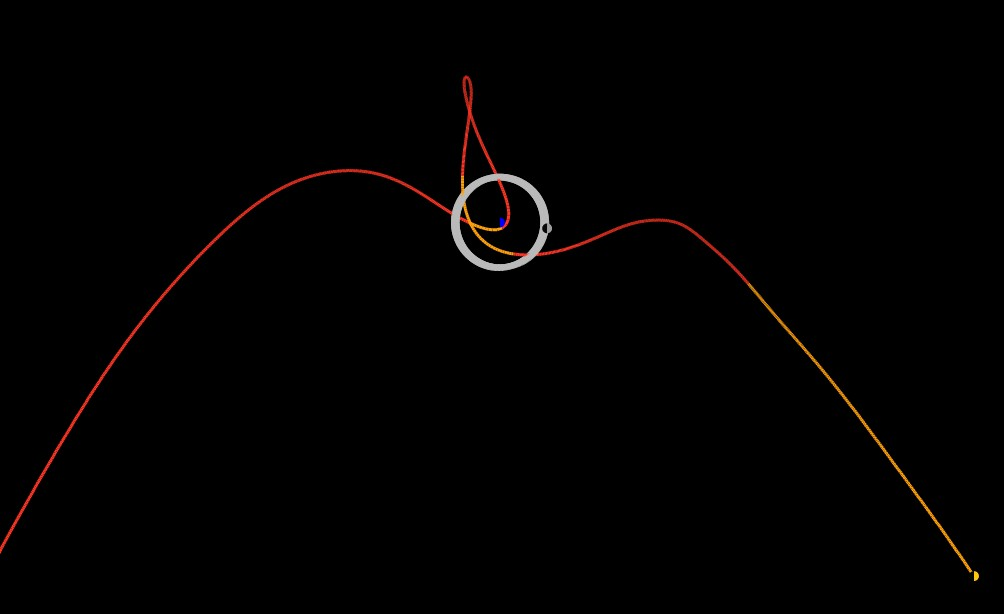
\includegraphics[width=\textwidth]{media/trajectories_2020SO.jpg}\\
		trajectories of objects in space \\
		\hyperref{https://en.wikipedia.org/wiki/2020_SO\#/media/File:2020SO_b.gif}{}{}{2020SO} 
	\end{minipage}
	\begin{minipage}[t]{0.25\textwidth}\centering
		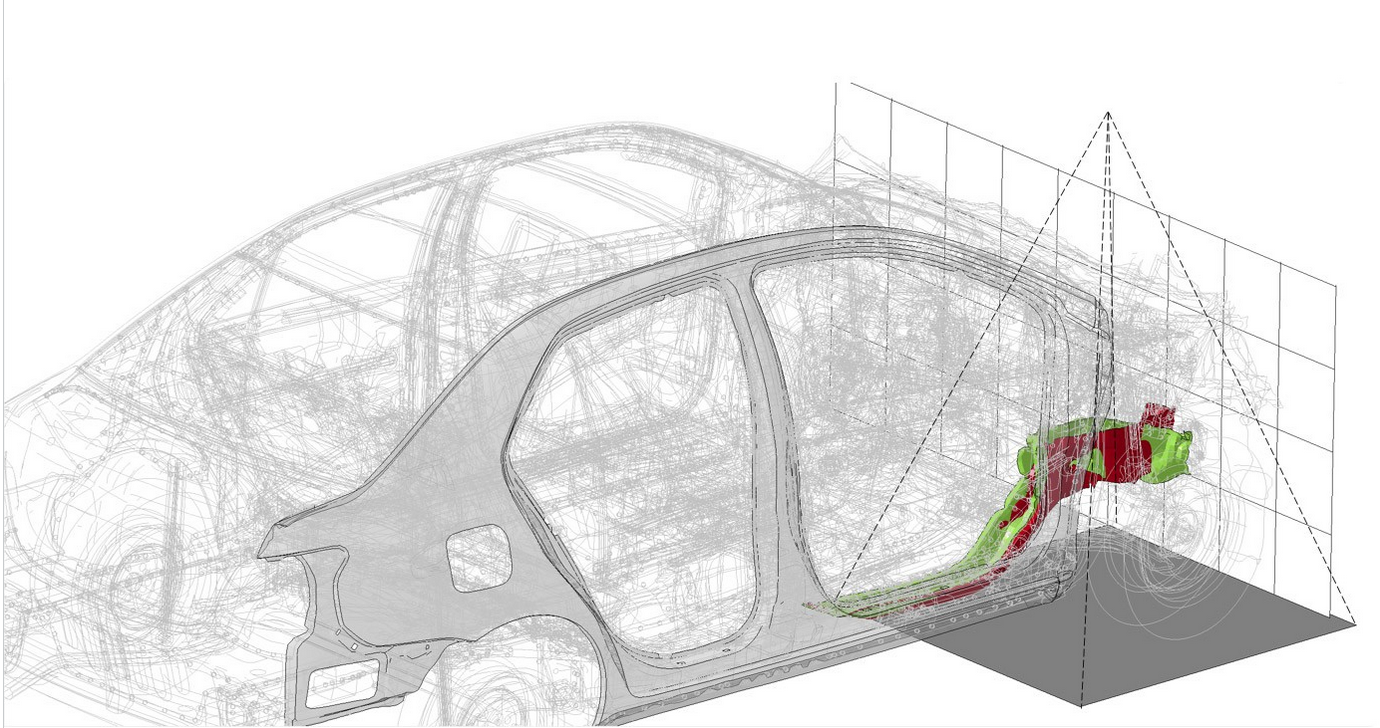
\includegraphics[width=\textwidth]{media/carcrash_sim.png}\\
		\hyperref{https://www.emi.fraunhofer.de/de/geschaeftsfelder/automotive/forschung/archiv/Roentgen-Crashtest.html}{}{}{car crash simulation} 
	\end{minipage}
	\begin{minipage}[t]{0.25\textwidth}\centering
		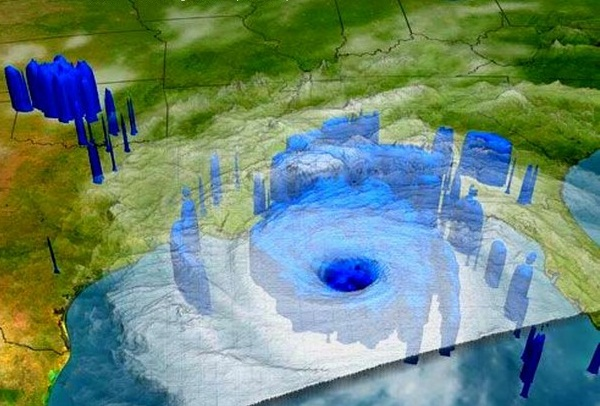
\includegraphics[width=\textwidth]{media/weather.jpg}\\
		\hyperref{https://en.wikipedia.org/wiki/Numerical_weather_prediction}{}{}{weather prediction} 
	\end{minipage}
	% CT SCAN
	\begin{minipage}[t]{0.25\textwidth} \centering
		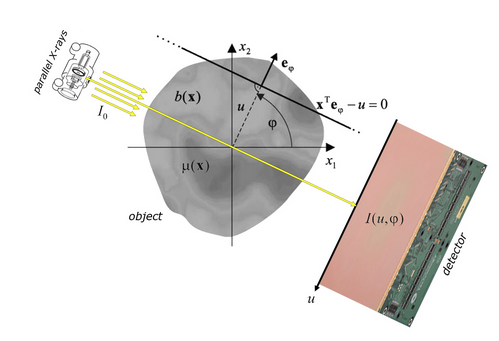
\includegraphics[width=\textwidth]{media/ct_scan.png}\\
		\hyperref{https://en.wikipedia.org/wiki/CT_scan}{}{}{CT Scan} 
	\end{minipage}
\end{frame}
%
\begin{frame}[c]
	\textbf{Relation to Data Science?}~\\
	\begin{itemize}
		\item due to the high amount of data available \textbf{data}-driven models are more important than ever \Vspace{0.2cm}
		\item data can be considered
		as a \textbf{mathematical object} (e.g., as a matrix/vector) \Vspace{0.2cm}
		\item with \textbf{numerical algorithms} we can manipulate data:\Vspace{0.2cm}
		\begin{itemize}\normalsize
			\item solve systems involving the data (fitting data, prediction,...)
			\vspace{0.2cm}\item extract the most important features (singular values, PCA, data compression,...) 
			\vspace{0.2cm}\item calibrate models against data (machine learning, neural networks,...)
		\end{itemize}
	\end{itemize}	
    \Vspace{2cm}
	\begin{minipage}[t]{0.25\textwidth}\centering
		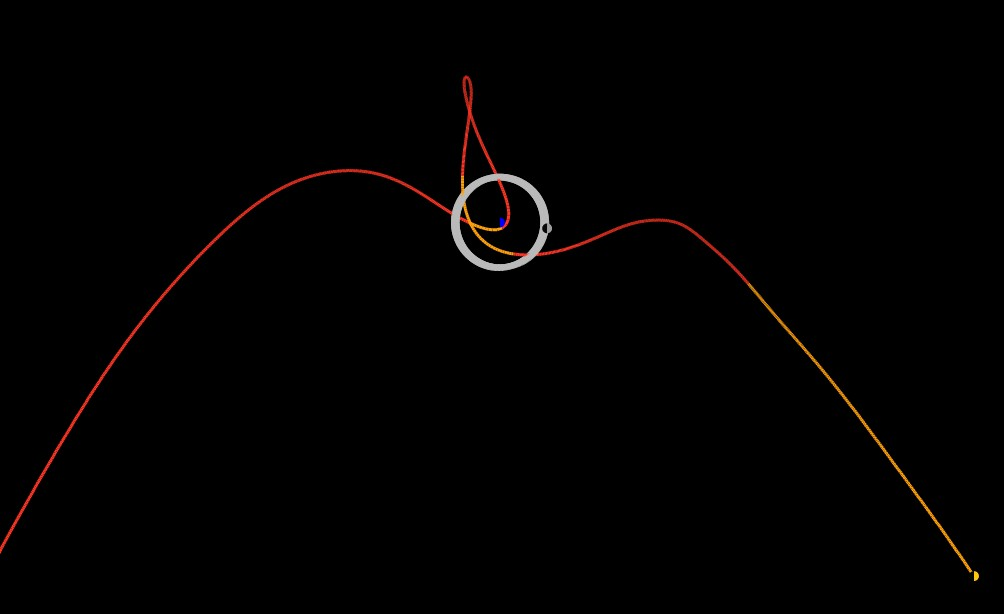
\includegraphics[width=\textwidth]{media/trajectories_2020SO.jpg}\\
		trajectories of objects in space \\
		\hyperref{https://en.wikipedia.org/wiki/2020_SO\#/media/File:2020SO_b.gif}{}{}{2020SO} 
	\end{minipage}
	\begin{minipage}[t]{0.25\textwidth}\centering
		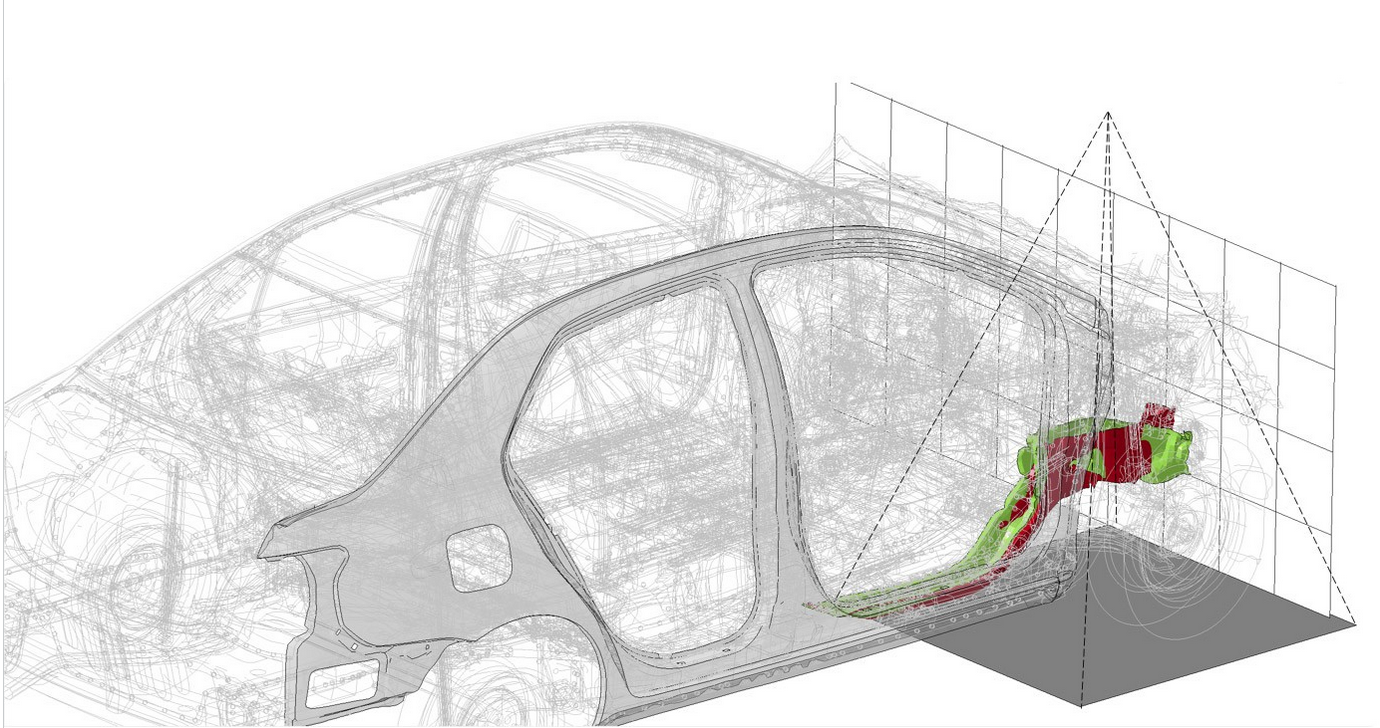
\includegraphics[width=\textwidth]{media/carcrash_sim.png}\\
		\hyperref{https://www.emi.fraunhofer.de/en/business-units/automotive/research/Roentgen-Crashtest.html}{}{}{car crash simulation} 
	\end{minipage}
	\begin{minipage}[t]{0.25\textwidth}\centering
		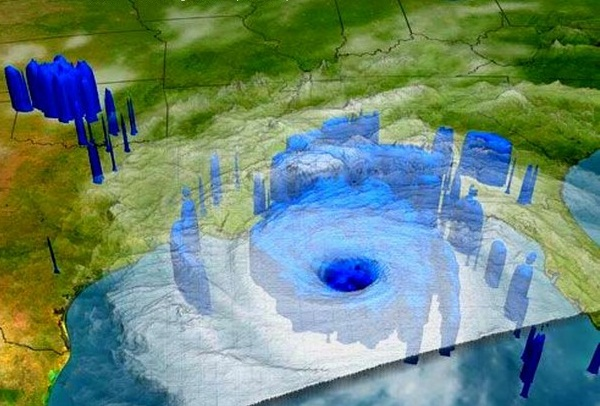
\includegraphics[width=\textwidth]{media/weather.jpg}\\
		\hyperref{https://en.wikipedia.org/wiki/Numerical_weather_prediction}{}{}{weather prediction} 
	\end{minipage}
	% CT SCAN
	\begin{minipage}[t]{0.25\textwidth} \centering
		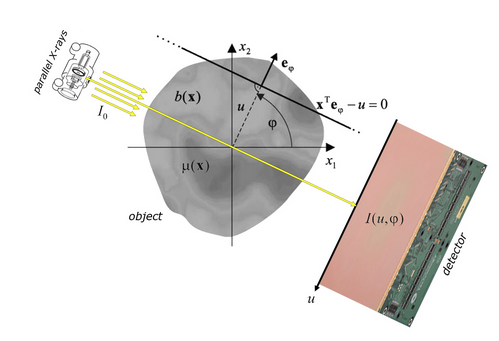
\includegraphics[width=\textwidth]{media/ct_scan.png}\\
		\hyperref{https://en.wikipedia.org/wiki/CT_scan}{}{}{CT Scan} 
	\end{minipage}
\end{frame}

%
\begin{frame}[c]
	\textbf{Preview}~\\
	\Vspace{0.25cm}
	Let us assume we have $m$ data points
	$$(z_i, y_i),~~~i=1,\ldots,m,$$
	where
	\begin{itemize}
		\item $z_i$ are $n$-dimensional vectors of \textit{explanatory features} 
		\item $y_i$ are $k$-dimensional vectors representing the \textit{response/prediction/classification}
	\end{itemize}
	~\\
	$\rightarrow$ \textit{The term \textit{``vector''} already indicates that Linear Algebra comes naturally into the game.}
	~\\~\\~\\
	\textbf{Examples}\\
	\begin{itemize}
		\item You ask $m$ persons about 
		\begin{align*}
		z_i &= (\text{age}, \text{sex},\text{weight},\text{height},\text{years of experience}) &(n=5 ~ \text{dimensional vector})\\
		y_i &= \text{salary} &(k=1 ~ \text{dimensional vector})
		\end{align*}
		\item Consider $m$ years where
		\begin{align*}
		z_i &= \text{year} &(n=1 ~ \text{dimensional vector})\\
		y_i &= \text{global mean temperature} &(k=1 ~ \text{dimensional vector})
		\end{align*}	
		\item Consider $m$ images that you want to classify 
		\begin{align*}
		z_i &=(p_{lj})_{lj} & (\text{image stored as matrix/vector})\\
		y_i &= (\text{dog}, \text{cat}, \text{elephant}) &(k=3 ~ \text{dimensional vector})
		\end{align*}
	\end{itemize}
	
\end{frame}

\begin{frame}[c]
	\textbf{\large  Dealing solely with the features $z$}~~\\~\\
	Applications of the \textbf{Singular Value Decomposition} are:\\
	% Consider just the $m$ $n$-dimensional feature vectors $z_i$:\\~\\
	~\\~\\
	\begin{minipage}[t]{0.48\textwidth}
		\textbf{Principal Component Analysis (PCA)}\\~\\
		{\raggedright
			$\rightarrow$ Aim: dimension reduction\\~\\}
		{\centering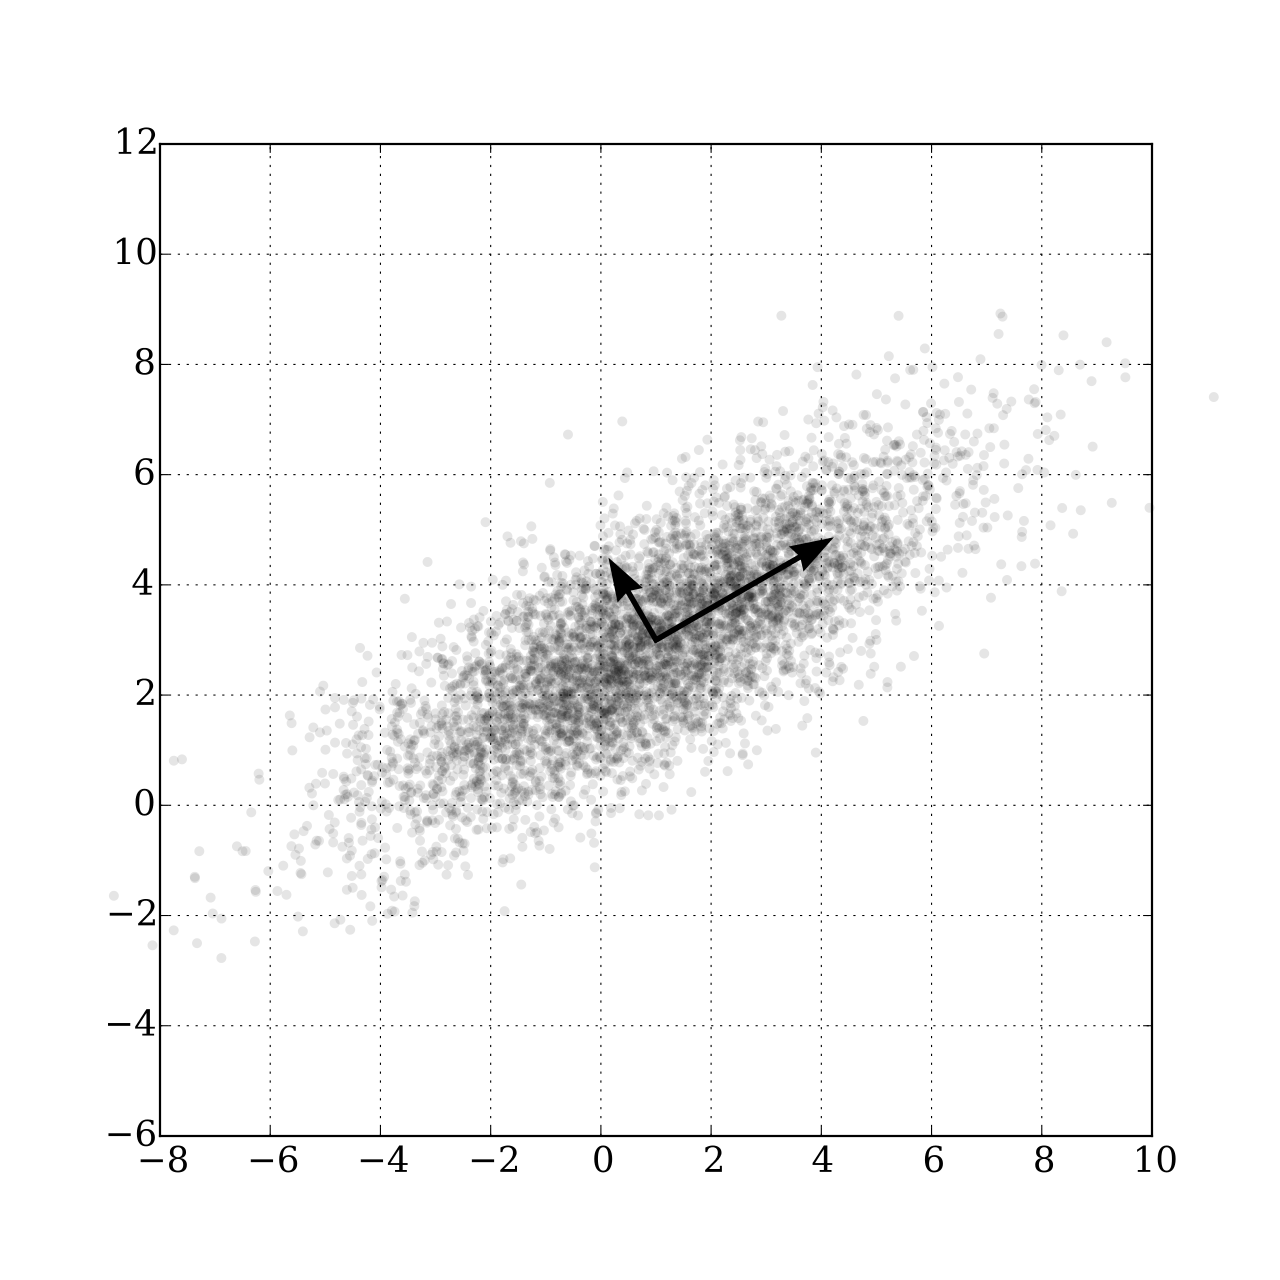
\includegraphics[width=0.77\textwidth]{media/PCA.png}}
	\end{minipage}
	~~~~~
	\begin{minipage}[t]{0.48\textwidth}
		\textbf{Data compression}\\~\\
		\raggedright
		$\rightarrow$ Aim: compression without dimension reduction\\~\\
		{ \hspace*{-0.6cm}\centering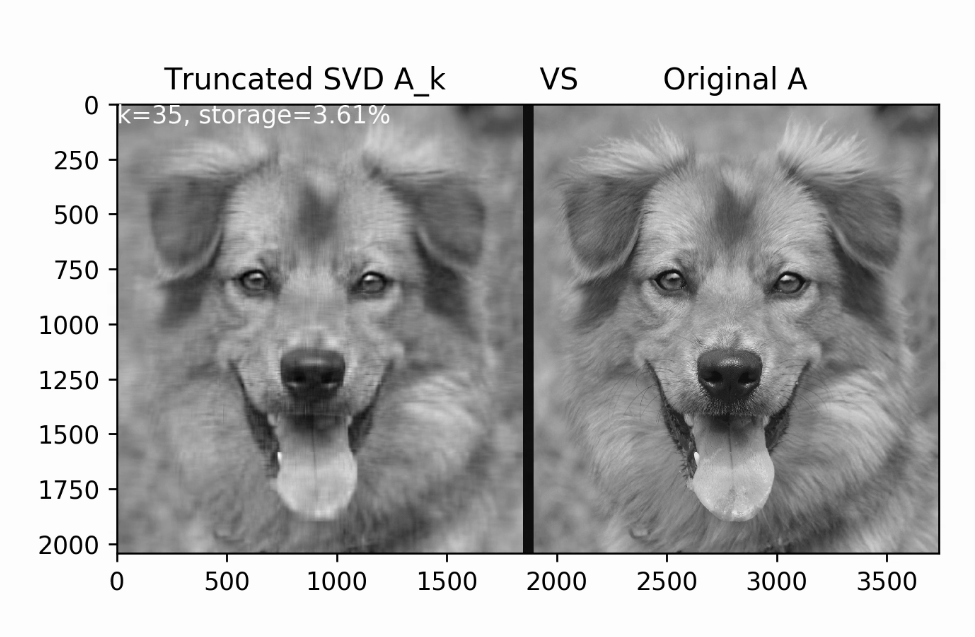
\includegraphics[width=1.1\textwidth]{media/SVD_dog.png}}
	\end{minipage}
\end{frame}
%
\begin{frame}[c]
	\textbf{\large  Relating features $z$ to response $y$}~\\~\\
	One central goal in many scientific fields is to find a \textbf{model} $f_x$ depending on some parameters $x=(x_i)_i$, which ``best'' explains the relation between $z_i$ and $y_i$ in the sense that 
	$$f_x(z_i) \approx y_i,~~~\text{for all}~~i=1,\ldots,m$$
	\begin{itemize}
		\item  \textbf{The task:} Find those parameters $x$ for which the ``distance'' between our prediction  $f_x(z_i)$ and the measured response $y_i$ is ``as small as possible''.\\
		\item Math gives us the tools to rigorously define this task, to analyze it systematically and to provide numerical solutions!
		~\\
	\end{itemize}
~\\
	\textbf{Curve Fitting}
		$$f_x(z) := x_0 + x_1z + x_2 z^2$$
		\\ \centering
		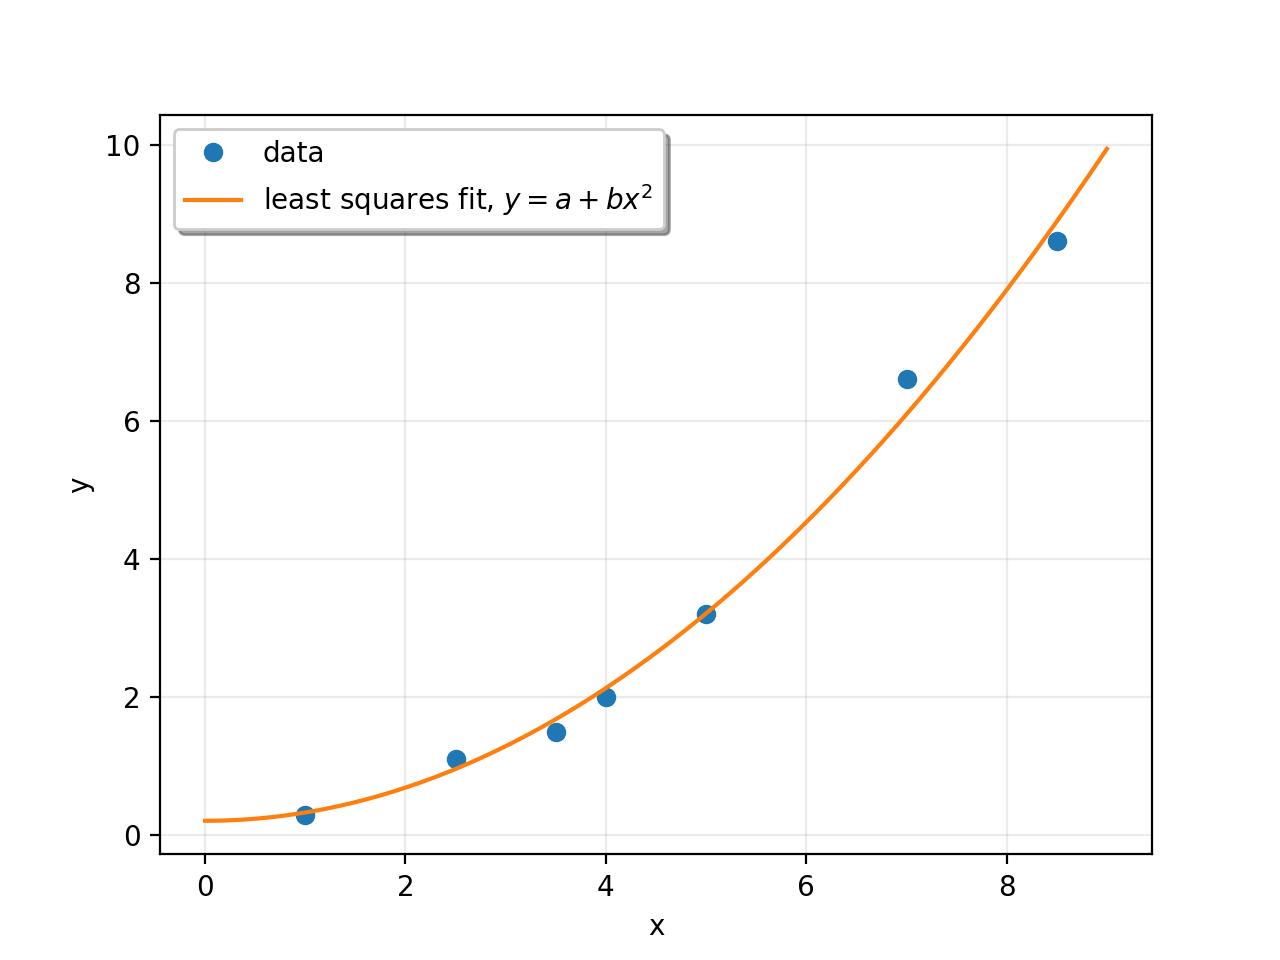
\includegraphics[width=0.37\textwidth]{media/4_least_squares.png}\\
\end{frame}

\begin{frame}[c]
	\textbf{Simple image inpainting}
	\vspace*{-0.3cm}
	$$\min_x \|Ax-b\|^2 + R(x)$$
	\begin{center}
		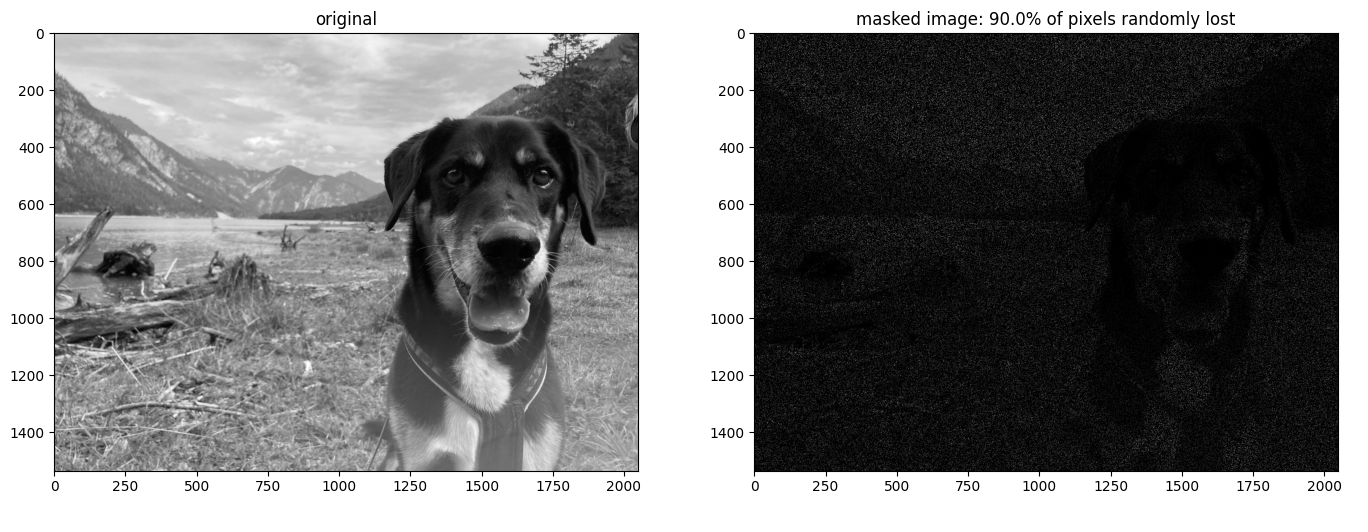
\includegraphics[width=0.8\textwidth]{media/Image_Inpainting-1.png}\\
		\vspace*{-0.3cm}
		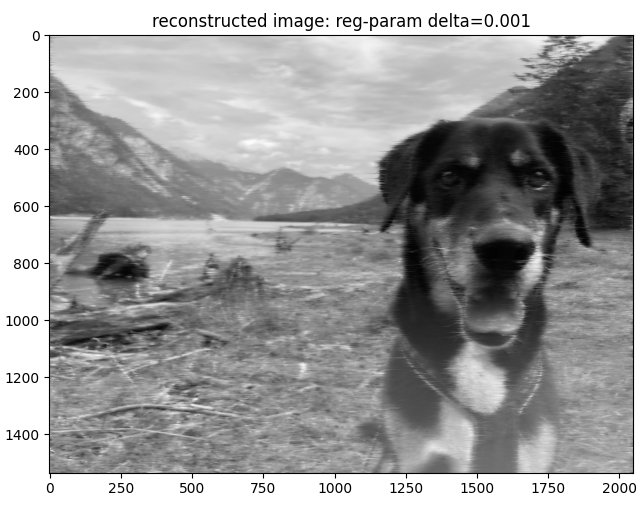
\includegraphics[width=0.45\textwidth]{media/Image_Inpainting-2.png}	
	\end{center}
\end{frame}

\begin{frame}[c]
\begin{center}
		 \begin{minipage}{0.8\textwidth}
		 \textbf{\Large Take away message}\\~\\
	 	Math provides a rigorous framework of abstract structures (Definition) within which their properties and relations (Theorem) can be systematically analyzed (Proof).
	 	~\\~\\
	 	The same mathematical concept can be exploited in multiple applications; see, e.g., SVD above.
	 	~\\~\\
	 	Given a real-world problem the user has to provide an interface (a mathematical model) to these  concepts to make use of the mathematical theory.
	 \end{minipage}
\end{center}
\end{frame}